% Topi whitepaper. Build with:  tectonic topi.tex   (or latexmk -xelatex topi.tex)
\documentclass[11pt,a4paper]{article}

\usepackage[margin=2.4cm,headheight=14pt]{geometry}
\usepackage{amsmath}
\usepackage{fontspec}
\usepackage{libertinus}
\usepackage{microtype}
\usepackage{xcolor}
\usepackage{booktabs,tabularx,array}
\usepackage{enumitem}
\usepackage{tikz}
\usetikzlibrary{arrows.meta,positioning,calc,fit,backgrounds}
\usepackage{titlesec}
\usepackage{fancyhdr}
\usepackage{caption}
\usepackage[hidelinks]{hyperref}

% The site's palette: red is a payment that can still be traced, amber a proof or a settled spend.
\definecolor{ink}{HTML}{0E0D0C}
\definecolor{inksoft}{HTML}{33302C}
\definecolor{mute}{HTML}{5C5852}
\definecolor{rule}{HTML}{CFCCC1}
\definecolor{paper}{HTML}{F4F3EE}
\definecolor{topired}{HTML}{FF4A24}
\definecolor{topiamber}{HTML}{F5B83D}
\hypersetup{colorlinks=true,linkcolor=inksoft,citecolor=topired,urlcolor=topired}

\titleformat{\section}{\Large\bfseries\color{ink}}{\color{topired}\thesection}{0.8em}{}
\titleformat{\subsection}{\large\bfseries\color{ink}}{\color{mute}\thesubsection}{0.7em}{}
\titleformat{\paragraph}[runin]{\bfseries\color{ink}}{}{}{}[.]
\titlespacing*{\section}{0pt}{2.2ex plus .5ex}{1.1ex}
\captionsetup{font=small,labelfont={bf,color=topired},labelsep=period}
\setlist{itemsep=2pt,topsep=4pt}
\renewcommand{\arraystretch}{1.15}
\setlength{\emergencystretch}{2em}

\pagestyle{fancy}
\fancyhf{}
\renewcommand{\headrulewidth}{0pt}
\fancyhead[L]{\small\color{mute}Topi: post-quantum private payments}
\fancyhead[R]{\small\color{mute}\thepage}

\newcommand{\code}[1]{\texttt{\small #1}}
\newcommand{\Hf}{\mathsf{H}}

\begin{document}

% ---------------------------------------------------------------- title
\thispagestyle{empty}
\begin{tikzpicture}[remember picture,overlay]
  \fill[ink] (current page.north west) rectangle ([yshift=-9.2cm]current page.north east);
  % a band of pixels thinning out, as between the website's sections
  \foreach \x in {0,...,104} {
    \foreach \r in {0,...,5} {
      \pgfmathsetmacro{\p}{(1-(\r+0.5)/6)^2.2}
      \pgfmathparse{rnd<\p ? 1 : 0}
      \ifnum\pgfmathresult=1
        \fill[ink] ([xshift=\x*0.2cm,yshift=-9.2cm-\r*0.2cm]current page.north west) rectangle ++(0.2cm,-0.2cm);
      \fi
    }
  }
  \fill[topired] ([xshift=7.4cm,yshift=-9.85cm]current page.north west) rectangle ++(0.14cm,-0.14cm);
  \fill[topiamber] ([xshift=14.1cm,yshift=-10.05cm]current page.north west) rectangle ++(0.14cm,-0.14cm);
  \node[anchor=north west,text=paper,font=\fontsize{46}{46}\selectfont\bfseries] at ([xshift=2.4cm,yshift=-2.6cm]current page.north west) {Topi};
  \node[anchor=north west,text=paper,text width=14cm,font=\Large] at ([xshift=2.4cm,yshift=-4.4cm]current page.north west)
    {Post-quantum private payments on Ethereum frame transactions};
  \node[anchor=north west,text=topiamber,font=\small] at ([xshift=2.4cm,yshift=-6.4cm]current page.north west)
    {Whitepaper, draft \quad\textbullet\quad \today};
\end{tikzpicture}
\vspace*{9.6cm}

\begin{abstract}
\noindent Private payment systems on Ethereum rest on elliptic curves almost everywhere: pairing-based
zero-knowledge proofs, elliptic-curve Diffie--Hellman in the packet formats of mixnets, and ECDSA for
every account and relayer. A large quantum computer breaks all three, and the confidentiality of traffic
recorded today can be broken after the fact. Topi is a private payment system in which no step on the
path from deposit to settlement depends on discrete logarithms. A wallet proves a withdrawal from a
shielded pool with a hash-based zero-knowledge proof and sends it through a three-hop mixnet whose
packets are sealed per hop with X-Wing, a hybrid of ML-KEM-768 and X25519. Admission to the mixnet is
rate limited by anonymous, hash-based epoch tickets. An exit node pairs spends and folds their proofs
by recursion into a single proof that an on-chain WHIR verifier checks; the pool settles both spends in
one EIP-8141 frame transaction authorized by leanSPHINCS, a hash-based signature scheme, so no ECDSA key
touches the pool. Settles reach the chain through an ERC-8421 alternative mempool that admits them by
the pool's own rules. A Lean~4 model of the pool's validation and settlement carries machine-checked
theorems and is tested transaction by transaction against the deployed contracts. Topi runs end to end
on a public test network: settles of two spends use about 16.3M gas, and a 1.3\,MB proof crosses four
cloud regions in about a minute over a mobile connection.
\end{abstract}

% ---------------------------------------------------------------- 1
\section{Introduction}

Privacy on a public ledger is a long-lived promise. A payment that is private today must remain private
for as long as anyone cares who paid whom, and the ledger keeps everything forever. This sets privacy
systems apart from most other cryptographic deployments: an adversary who records data now and breaks
the underlying assumption later still wins. For systems built on the hardness of the discrete logarithm,
that later adversary is a cryptographically relevant quantum computer running Shor's
algorithm~\cite{shor}.

Today's private payment designs for Ethereum depend on elliptic curves in three places:
\begin{itemize}
  \item \textbf{Proofs.} Shielded pools typically use Groth16~\cite{groth16} over the BN254 pairing curve.
    A quantum adversary who recovers the discrete logarithms in its structured reference string can
    forge proofs and drain the pool.
  \item \textbf{Transport.} Mixnets in the Sphinx~\cite{sphinx} family derive per-hop keys by
    elliptic-curve Diffie--Hellman. Traffic recorded today can be unwrapped once those keys fall,
    revealing who sent which message.
  \item \textbf{Authorization.} Every deposit, relayer and fee payment is signed with ECDSA, whose keys a
    quantum adversary recovers from public keys exposed on chain.
\end{itemize}

Topi replaces each of these. Its contributions are:
\begin{enumerate}
  \item a shielded pool that runs as an EIP-8141~\cite{eip8141} account, settles two spends per
    transaction with one hash-based recursive proof, and binds that proof to the spends' public fields
    on chain;
  \item a KEM-based Sphinx mixnet with an X-Wing~\cite{xwing} encapsulation per hop, fixed 8\,KB packets,
    batching, cover traffic and single-use reply blocks;
  \item anonymous per-epoch rate limiting from Binius64~\cite{binius} zero-knowledge proofs over
    SHA-256, with no pairings and no trusted setup;
  \item post-quantum authorization of every transaction on the pool path with leanSPHINCS signatures in
    EIP-8141 signature entries, for user accounts and for the paymaster that pays for settles;
  \item an ERC-8421~\cite{erc8421} alternative mempool for settles, which the public mempool cannot
    carry, run on the reference sidecar with a per-mempool validation budget and the pool's own
    admission rules;
  \item a Lean~4~\cite{lean4} model of the pool's validation and settlement with machine-checked safety
    theorems, checked against the chain by differential testing;
  \item an implementation running end to end on a public test network, with measurements.
\end{enumerate}

% ---------------------------------------------------------------- 2
\section{Background}

\paragraph{Frame transactions} EIP-8141 introduces a transaction type that is a list of
\emph{frames} executed in order, each with a mode, a target, gas limits and data, plus a list of
signature entries. A \code{VERIFY} frame calls an account's validation code, which approves the
transaction with a scope: \code{PAYMENT} makes the account pay for gas, \code{EXECUTION} lets later
\code{SENDER} frames act as the sender. Validation reads the transaction through new opcodes, so any
account can define its own authorization. A signature entry of scheme \code{ARBITRARY} carries opaque
bytes that the validating account interprets; the signature hash covers the whole transaction except the
bytes of entries whose message is empty, so a witness in such an entry can sign the entire transaction,
including the frame that verifies it.

\paragraph{Privacy Pools} The withdrawal relation of Privacy Pools~\cite{privacypools} proves that a
withdrawal spends a note committed in a pool tree, whose deposit label lies in an association tree, and
reveals a nullifier that prevents a second spend. Topi uses this relation with a change note, so a
withdrawal can take part of a note's value.

\paragraph{Hash-based proofs} Spartan~\cite{spartan} reduces circuit satisfiability to sum-checks; WHIR
\cite{whir} is a hash-based polynomial commitment and proximity test with fast verification. Both rest
only on collision-resistant hashing and are plausibly post-quantum. leanVM is a minimal zkVM built for
recursively verifying such proofs.

\paragraph{Post-quantum primitives} ML-KEM~\cite{fips203} is the lattice-based key encapsulation
standardized by NIST; X-Wing~\cite{xwing} combines ML-KEM-768 with X25519 so that the result is secure if
either component is. SPHINCS+~\cite{sphincs,fips205} is a stateless hash-based signature scheme;
leanSPHINCS is a variant over Keccak with an on-chain verifier.

% ---------------------------------------------------------------- 3
\section{System overview}

Topi has five parts: a wallet (the SDK and a client prover), a post-quantum mixnet of four roles, an
exit prover that aggregates spends, an alternative mempool for settles, and contracts on chain. Figure~\ref{fig:arch} shows the path of one
spend. The mixnet carries only proofs and their public fields; the exit learns which spends it pairs,
but not who sent them.

\begin{figure}[ht]
\centering
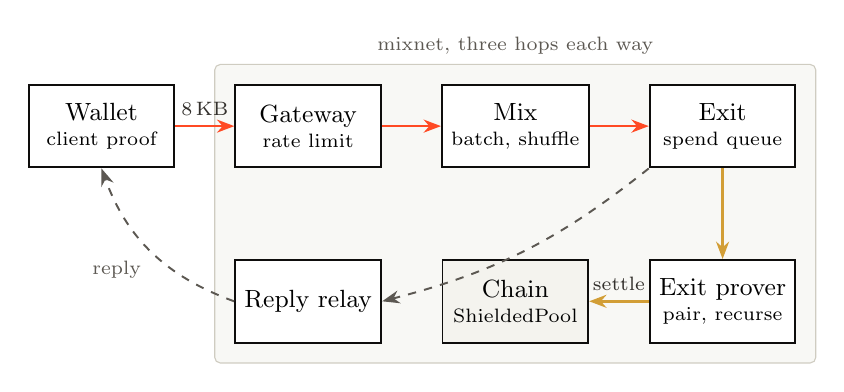
\begin{tikzpicture}[
  node distance=0.55cm and 0.75cm,
  box/.style={draw=ink,line width=0.7pt,fill=white,minimum height=1.05cm,minimum width=1.85cm,align=center,font=\small},
  fwd/.style={-{Stealth[length=2.2mm]},line width=0.9pt,topired},
  rep/.style={-{Stealth[length=2.2mm]},line width=0.7pt,mute,dashed},
  set/.style={-{Stealth[length=2.2mm]},line width=0.9pt,topiamber!85!ink}]
  \node[box] (w) {Wallet\\[-2pt]\scriptsize client proof};
  \node[box,right=of w] (g) {Gateway\\[-2pt]\scriptsize rate limit};
  \node[box,right=of g] (m) {Mix\\[-2pt]\scriptsize batch, shuffle};
  \node[box,right=of m] (e) {Exit\\[-2pt]\scriptsize spend queue};
  \node[box,below=1.15cm of e] (p) {Exit prover\\[-2pt]\scriptsize pair, recurse};
  \node[box,below=1.15cm of m,fill=paper] (c) {Chain\\[-2pt]\scriptsize ShieldedPool};
  \node[box,below=1.15cm of g] (r) {Reply relay};
  \draw[fwd] (w) -- node[above,font=\scriptsize,text=inksoft]{8\,KB} (g);
  \draw[fwd] (g) -- (m);
  \draw[fwd] (m) -- (e);
  \draw[set] (e) -- (p);
  \draw[set] (p) -- node[above,font=\scriptsize,text=inksoft]{settle} (c);
  \draw[rep] (e.south west) to[bend left=12] (r.east);
  \draw[rep] (r.west) to[bend left=25] node[below left,font=\scriptsize,text=mute]{reply} (w.south);
  \begin{scope}[on background layer]
    \node[fit=(g)(m)(e)(r),draw=rule,fill=paper!60,rounded corners=2pt,inner sep=7pt,
      label={[font=\scriptsize,text=mute]above:mixnet, three hops each way}] {};
  \end{scope}
\end{tikzpicture}
\caption{The path of a spend. Red: the forward route, on which a payment can still be traced to its
sender's network address until it has crossed the mix. Amber: the exit's aggregation and the settle.
Dashed: the reply on a single-use reply block.}
\label{fig:arch}
\end{figure}

\noindent The lifecycle of a private spend is:
\begin{enumerate}
  \item \textbf{Deposit.} A post-quantum account calls \code{deposit} with value and a precommitment
    only it can open; the pool inserts the note.
  \item \textbf{Prove.} The wallet rebuilds the pool's trees from its events and proves a withdrawal in
    zero knowledge: about a second and 450\,MB.
  \item \textbf{Send.} The 1.3\,MB proof and its fields leave as about 280 packets of 8,192 bytes through
    gateway, mix and exit, admitted on one anonymous rate-limit token.
  \item \textbf{Aggregate.} The exit checks each queued spend against the chain, pairs two, and folds
    both proofs by recursion into one terminal proof: about 19 minutes and 12\,GB on a laptop, or
    151\,s on a 32-vCPU cloud instance.
  \item \textbf{Settle.} One frame transaction with the pool as sender verifies the terminal proof,
    binds it to both spends, consumes both nullifiers, pays the recipients and inserts the change notes.
    The exit prover submits it to the alternative mempool (Section~\ref{sec:mempool}), which checks it,
    gossips it between nodes and relays it to the chain.
\end{enumerate}

% ---------------------------------------------------------------- 4
\section{The shielded pool}\label{sec:pool}

\subsection{Fields and digests}
All hashing is over the KoalaBear prime field, $p = 2^{31} - 2^{24} + 1 = 2{,}130{,}706{,}433$. A digest
is eight field elements; on chain it is packed into one 256-bit word. Every element entering the
contract is checked to be below $p$. We write $\Hf_D(x_1 \| \dots \| x_n)$ for the Poseidon2~\cite{poseidon2}
sponge over KoalaBear with domain tag $D$.

\subsection{Deposits}
A deposit carries value $v < 2^{128}$ and a precommitment
$\mathit{pre} = \Hf_{\textsc{precommit}}(\mathit{nullifier} \,\|\, \mathit{secret})$. The pool assigns the
next index and computes
\begin{align*}
  \mathit{label} &= \Hf_{\textsc{label}}(\mathit{scope} \,\|\, \mathit{index}), \\
  \mathit{note}  &= \Hf_{\textsc{note}}(\mathit{pool} \,\|\, \mathit{label} \,\|\, v \,\|\, \mathit{pre}),
\end{align*}
inserting $\mathit{note}$ (as a pair, so later paired inserts stay aligned) into the pool tree and
$\mathit{label}$ into the association tree. Both are depth-32 incremental Merkle trees; every root either
tree has had is recorded, and a spend may prove against any recorded root. The deposit event carries
every leaf, so a wallet can rebuild both trees from logs alone.

\subsection{Spends}
A spend is described by 82 public fields: pool and scope identity, a \emph{context} that commits to the
fee recipient, the recipient, the withdrawn amount, the fee, the pool and association roots, the
nullifier hash and the change-note commitment. The client proof shows that these fields describe a valid
withdrawal; its only public input is the transaction digest $\Hf_{\textsc{tx}}(\mathit{fields})$.

\subsection{Settlement}
The exit prover submits one frame transaction whose sender is the pool (Table~\ref{tab:settle}).

\begin{table}[ht]
\centering\small
\begin{tabularx}{\linewidth}{@{}clllX@{}}
\toprule
Frame & Mode & Target & Scope & Effect \\
\midrule
0 & \code{VERIFY} & pool & execution & the pool's policy approves exactly this shape \\
1 & \code{VERIFY} & paymaster & payment & checks the exit operator's leanSPHINCS signature, pays gas \\
2 & \code{SENDER} & pool & & \code{settle(proofCall, a, b)}: verification and state change \\
\bottomrule
\end{tabularx}
\caption{The settle transaction. The pool never pays gas, and only \code{settle} ever runs as the pool.}
\label{tab:settle}
\end{table}

\noindent \code{settle} requires that it runs as the pool; forwards the proof to the terminal verifier
and requires acceptance; recomputes the application root from both spends' fields and requires it to
equal the root inside the proof calldata; checks that each spend names this pool and known roots and an
unspent nullifier, and marks it spent; inserts both change notes; pays each recipient and the committed
fee recipient; and emits \code{Settled}. Any failure reverts the \code{SENDER} frame, so no nullifier is
consumed and no value moves.

\subsection{Design decisions}
\begin{itemize}
  \item \textbf{Nullifiers in storage, not in nonce keys.} Were a nonce key required to equal a
    nullifier, an attacker could copy a pending spend's nullifier into a transaction with a bogus proof:
    validation would pass and consume the key, \code{settle} would revert, and the victim's note would
    become unspendable. With storage nullifiers a failed settle consumes nothing.
  \item \textbf{The fee goes to the committed address.} A front-runner who copies a valid proof can only
    execute the victim's own withdrawal; it cannot redirect the fee.
  \item \textbf{Fresh random nonce keys.} Each settle uses a random 128-bit nonce key, so spends are
    order-free and can be delayed by the mixnet without a shared nonce queue.
  \item \textbf{Heavy work in the \code{SENDER} frame.} Validation is capped at 500,000 gas, far below the
    cost of verifying a proof.
\end{itemize}

% ---------------------------------------------------------------- 5
\section{Proofs and recursion}

\paragraph{Client proof} Each spend is proven with Spartan-WHIR in full zero knowledge over a circuit of
63,952 constraints for the Privacy Pools relation with change. Proving takes about a second and 450\,MB
on a laptop; the proof is about 1.3\,MB.

\paragraph{Recursion} The exit runs leanVM over two client proofs: it verifies each inside the VM,
lifts them, and runs a grouped root recursion. The output is a grouped Keccak WHIR terminal proof of
about 100\,KB, whose \emph{application root} commits to both spends' statements.

\paragraph{Binding on chain} The generated terminal verifier returns only a boolean: some two proofs
with statements hashing to the application root were accepted by the fixed programs. It does not see
public inputs. The pool therefore recomputes, for each spend,
\begin{align*}
  d &= \Hf_{\textsc{tx}}(\mathit{fields}_{0..81}), \\
  s &= \mathrm{P1}\big(\texttt{"leanvm-spartan-whir-statement-v1"},\, d\big),
\end{align*}
where $\Hf$ is Poseidon2 and $\mathrm{P1}$ a length-prefixed Poseidon1 digest, and the root $\mathrm{P1}(\textsc{nod1}, 2, s_A, s_B)$, and requires it to equal the proven application
root. This binding is what ties an otherwise generic proof to these two spends. Terminal verification
costs about 10.2M gas with its calldata; a full settle about 16.3M, of the $2^{24}$ per-transaction cap.

% ---------------------------------------------------------------- 6
\section{The mixnet}

\subsection{Packet format}
Topi's packets are a KEM-based variant of Sphinx. Instead of one group element blinded per hop, each hop
receives its own X-Wing ciphertext, so a packet stays confidential if either ML-KEM-768 or X25519 holds.
From each hop's shared secret, BLAKE3 derives four keys: header MAC, header stream, payload stream and
replay tag. The header uses the Sphinx filler construction, so its length is the same at every hop, and
every node keeps the replay tags it has seen and drops repeats.

\begin{figure}[ht]
\centering
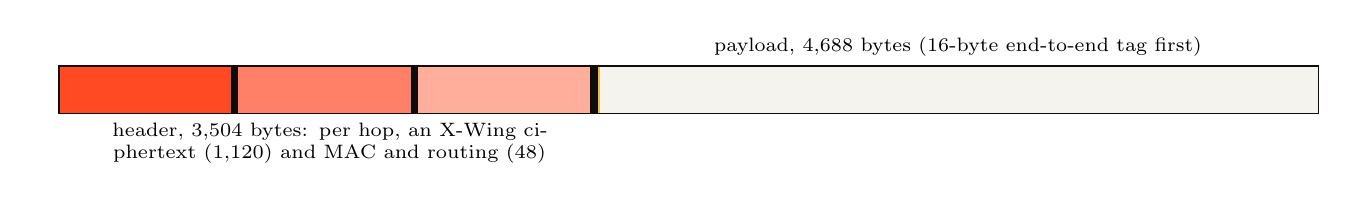
\begin{tikzpicture}[x=0.00195cm,y=1cm,font=\scriptsize]
  \foreach \i/\c in {0/topired,1/topired!70,2/topired!45} {
    \fill[\c] ({\i*1168},0) rectangle ++(1120,0.6);
    \fill[ink] ({\i*1168+1120},0) rectangle ++(48,0.6);
  }
  \fill[topiamber] (3504,0) rectangle ++(16,0.6);
  \fill[paper] (3520,0) rectangle (8192,0.6);
  \draw[ink,line width=0.5pt] (0,0) rectangle (8192,0.6);
  \draw[ink,line width=0.5pt] (3504,0) -- (3504,0.6);
  \node[below,text width=7.4cm,align=center] at (1752,0) {header, 3,504 bytes: per hop, an X-Wing ciphertext (1,120) and MAC and routing (48)};
  \node[above] at (5848,0.6) {payload, 4,688 bytes (16-byte end-to-end tag first)};
\end{tikzpicture}
\caption{Every packet is 8,192 bytes at every hop.}
\end{figure}

\subsection{Roles and routes}
The forward route is always gateway, mix, exit. Routes are drawn at random from the nodes the topology
lists for each role: one gateway per session (it holds the client's epoch ticket), one exit per message
(it reassembles the message), and a fresh mix per packet. The gateway delays each packet by an exponentially
distributed time (mean 100\,ms), as in Loopix~\cite{loopix}; the mix ignores per-packet delay and instead
collects packets for a batch interval (1.5\,s by default) and releases each batch shuffled. The gateway
also emits cover packets at exponential intervals (mean 700\,ms), indistinguishable from real packets
until the exit removes the last layer.

\subsection{Messages and replies}
A message larger than one payload is split into fragments; the first also carries a single-use reply
block (SURB) for the route reply relay, mix, gateway, whose last routing entry names a random reply slot.
The exit reassembles the message, queues the spend, and answers on the SURB; the reply waits in the
gateway's reply store until the client polls for it. Clients never accept inbound connections, so they
work behind NAT and on mobile networks.

% ---------------------------------------------------------------- 7
\section{Anonymous rate limiting}

A gateway must refuse floods without learning who sends what. Each registered member may send $L = 16$
messages per epoch of 600\,s. With member secret $\mathit{sk}$:
\begin{align*}
  C &= \mathrm{SHA256}(\texttt{"TPID"} \,\|\, \mathit{sk}), & M &= \mathrm{MerkleRoot}(\{C\}), \\
  t_i &= \mathrm{SHA256}(\texttt{"TPTK"} \,\|\, \mathit{sk} \,\|\, \mathit{epoch} \,\|\, i), & R &= \mathrm{MerkleRoot}(t_0, \dots, t_{L-1}),
\end{align*}
for $0 \le i < L$, where $M$ is published.
Once per epoch the client proves in zero knowledge that it knows $\mathit{sk}$ and a path placing $C$
under $M$, and that $R$ is the token root for $(\mathit{sk}, \mathit{epoch})$; only $(M, \mathit{epoch}, R)$
are public. The proof is a Binius64 proof wrapped in an outer zero-knowledge Spartan proof: 79 SHA-256
compressions, about 316\,KiB, proven in about 0.2\,s and verified in about 0.19\,s. Each message then
carries a token $(t_i, i, \text{path to } R)$ of 164 bytes, and the gateway accepts each $t_i$ once.
Because $R$ is a deterministic function of $(\mathit{sk}, \mathit{epoch})$ and has only $L$ leaves, over-use
is impossible rather than punishable.

A spend is about 280 packets, so a message spends one token on its first packet and receives a budget of
512 continuation packets that carry only the 32-byte token value.

% ---------------------------------------------------------------- 8
\section{Post-quantum authorization}

Every transaction on the pool path is authorized by leanSPHINCS: signatures of 5,684 bytes under a public
key of two 32-byte words, checked by a shared verifier contract.
\begin{itemize}
  \item \textbf{Accounts.} A user account is a two-frame transaction: a \code{VERIFY} frame on the account
    approving both execution and payment, and a \code{SENDER} frame with the call. One empty-message
    \code{ARBITRARY} entry holds the witness over the signature hash. Wallets deposit from such accounts
    and receive withdrawals to them.
  \item \textbf{The paymaster.} The post-quantum paymaster approves payment only for transactions of its
    pool that carry exactly one \code{ARBITRARY} entry accepted under the exit operator's key. Its
    \code{VERIFY} frame costs about 61,000 gas.
\end{itemize}
Account and paymaster validation must run opcodes that Solidity cannot emit, so both are written in Yul.

% ---------------------------------------------------------------- 9
\section{An alternative mempool for settles}\label{sec:mempool}

A settle cannot enter the public mempool of an EIP-8141 chain, for two reasons. Every settle has the same
sender, the pool, and the same paymaster, while the public mempool keeps one pending transaction per
sender and per non-canonical paymaster. And its validation prefix declares 160,100 gas (the pool's
\code{VERIFY} frame 10,000, the post-quantum paymaster 150,000, the signature entry 100), above the public
limit of 100,000. ERC-8421~\cite{erc8421} lets a set of nodes run an alternative mempool with its own
admission rules, identified by the hash of the document that defines them.

\paragraph{Design} The topi privacy-pool mempool is defined by a rules document whose IPFS CIDv0 is its
id. It runs on the ERC-8421 reference sidecar, a fork of the skandha bundler for frame transactions,
pinned to one commit and extended by a patch:
\begin{itemize}
  \item a validation budget per mempool (200,000 here, against the fixed 100,000);
  \item a pluggable admission policy, run at admission and on every block, that applies the pool's rules
    and reports its verdict as one more rule;
  \item nodes without an ERC-7562 tracer: chain 8141's client has none, so such a node simulates
    validation untraced and admits only whitelisted entities (the pool and its paymaster), and the policy
    stands in for the opcode and storage rules;
  \item the 8-field transaction encoding of chains without EIP-8272 recent-root references, relay through
    \code{eth\_sendRawTransaction}, and a duplicate relay treated as success;
  \item a gossip frame-data limit of 128\,KiB instead of 64,000 bytes. A settle is about 104\,KB; the
    original limit dropped it silently.
\end{itemize}
Clients submit with \code{eth\_sendFrameTransaction}, the transaction as JSON, and a refusal names the rule
it broke. Two nodes gossip over libp2p.

\paragraph{Rules} A node admits a settle when it has the three frames of Table~\ref{tab:settle} with no
value and no blobs and a fresh nonce key; one \code{ARBITRARY} entry of 5,684 bytes that verifies under the
exit's leanSPHINCS key; a validation budget of at most 200,000; two spends that name this pool and scope,
pay the fee to the transaction's fee recipient, carry distinct nullifiers unspent on chain and not claimed
by another pending settle, and cite known roots; pool and paymaster code unchanged since the node started;
and an approving simulation. At most 256 settles are pending, 64 per paymaster, each for at most
30 minutes, and every block re-checks them.

\paragraph{Staking} ERC-8421 nodes read stakes from a staking registry, deployed on chain 8141 for this
purpose. Staking is keyed on the caller, and the deployed pool account and paymaster have no call that
stakes, so they remain whitelisted entities rather than staked ones.

\paragraph{Results} Five settles on chain 8141 went through the sidecar and were mined, in blocks 717,928,
719,307, 720,937, 721,379 and 721,480. In the last, the second node received the settle from the first by
gossip and passed all ten of its checks itself. Submission to inclusion takes about 20\,s. On the
organizers' public ERC-8421 devnet, which applies the standard rules with full ERC-7562 tracing and no
custom policy, a post-quantum settle passed 24 of 24 admission checks and was mined in block 8,944. That
devnet's 60M block gas limit and about 1,530 state gas per byte of code cap deployable code at about
37\,KB, so the 59\,KB terminal verifier and the 50\,KB pool logic cannot be deployed there. The settle
there used the real pool account, post-quantum paymaster (validation limit 95,000, within the unstaked
per-entity budget) and leanSPHINCS verifier, with a stand-in logic that checks pool and scope and records
nullifiers but does not verify the proof; proofs are verified on chain 8141.

\section{Formal verification}

A Lean~4 model transcribes the pool account's and both paymasters' validation, and the settlement state
machine. Among its machine-checked theorems:
\begin{itemize}[before=\raggedright]
  \item an approved pool transaction has exactly three frames, and only \code{settle} runs as the pool
    (\code{only\_settle\_runs\_as\_pool});
  \item the pool never pays for its own transactions (\code{pool\_never\_pays});
  \item no nullifier is spent twice over any history of transactions (\code{run\_distinct});
  \item a settle that fails changes nothing (\code{failed\_settle\_changes\_nothing});
  \item the pool's balance always equals the value of its live notes (\code{settle\_preserves\_inv});
  \item with the post-quantum paymaster, no signature on the pool path is ECDSA
    (\code{pq\_pool\_tx\_has\_no\_ecdsa}).
\end{itemize}
All proofs depend only on Lean's \code{propext} and \code{Quot.sound}; continuous integration fails if
any depends on \code{sorryAx} or \code{Classical.choice}. The model abstracts the cryptography and
assumes proof-system soundness. The alternative mempool and the devnet's stand-in settle logic are
outside it, and the model is unchanged by them. Its correspondence to deployed bytecode is checked by
differential tests
against the chain: 528 of 528 cases for the pool policy with the classic paymaster, 90 of 90 with the
post-quantum paymaster, 56 of 56 regression cases and 42 of 42 for the post-quantum account.

% ---------------------------------------------------------------- 10
\section{Security}

\begin{table}[ht]
\centering\small
\begin{tabularx}{\linewidth}{@{}>{\raggedright}p{3.9cm}>{\raggedright}p{3.6cm}X@{}}
\toprule
Property & Against & Provided by \\
\midrule
Deposit--withdrawal unlinkability & chain observers & zero-knowledge client proof; nullifiers reveal nothing about the note \\
Sender's network identity & the exit, the RPC, partial network observers & three hops, fixed-size packets, batching, cover traffic \\
Gas-payment unlinkability & chain observers & the pool is the sender; a paymaster pays \\
Pool funds & anyone submitting transactions & validation policy, statement binding, storage nullifiers, the Lean model \\
Long-term confidentiality and authorization & a future quantum adversary & X-Wing, hash-based proofs, leanSPHINCS \\
\bottomrule
\end{tabularx}
\caption{What Topi protects, and how.}
\end{table}

\paragraph{Trust} The exit operator is trusted for liveness, not safety: it can refuse or delay spends but
cannot redirect funds, because recipients and the fee recipient are fixed by the proof and the binding
check. The mixnet gives anonymity if at least one hop is honest and there is enough concurrent traffic for
batches to mix. The paymaster risks only gas.

\paragraph{Limitations} Topi is research software on a test network and has not been audited.
\begin{itemize}
  \item Routes are random, but with one node per role there is only one choice, so a single compromised
    mix or a global observer of all links defeats mixing; with little traffic, batches are small.
  \item On chain 8141 the mempool cannot trace validation, so it relies on a whitelist and its own policy
    in place of the ERC-7562 opcode and storage rules.
  \item The payload uses a per-hop stream layer rather than a wide-block cipher, so payload tagging is
    detected only end to end.
  \item A member's tokens within one epoch are linkable at the gateway, and continuation token values
    travel in the clear to it.
  \item A settle needs exactly two spends; the exit sees the public fields of the spends it pairs.
  \item Upstream reports that the recursion's full composition security is not yet established; the proof
    systems and leanSPHINCS are young implementations.
  \item Funding a post-quantum account, the fee recipient and the paymaster's admin withdrawal still use
    classical accounts, and Ethereum's consensus is not post-quantum.
\end{itemize}

% ---------------------------------------------------------------- 11
\section{Evaluation}

Measurements come from a 16-thread laptop and from transactions on the chain~8141 test network.

\begin{table}[ht]
\centering\small
\begin{tabular}{@{}lr@{}}
\toprule
Measurement & Value \\
\midrule
Packet construction / processing per hop & 0.4\,ms / 0.18\,ms \\
Ping round trip across four AWS regions & 3.8 to 10\,s \\
1.3\,MB spend over a mobile uplink, queued at the exit & 68 to 78\,s \\
Epoch ticket: prove / verify & 0.2\,s / 0.19\,s \\
Client proof: prove / peak memory & about 1\,s / 450\,MB \\
Exit recursion of two proofs, laptop & 721 to 1,150\,s, 12.4\,GB \\
Exit recursion, 32-vCPU cloud instance (warm / fresh) & 151\,s / 210 to 332\,s \\
Two notes to a mined settle, recursion in the cloud & 216 to 301\,s \\
Settle through the alternative mempool, to inclusion & about 20\,s \\
\midrule
Poseidon2-24 permutation on chain & 68,600 gas \\
Terminal proof verification with calldata & 10.2M gas \\
Deposit from a post-quantum account & 7.5M gas \\
Settle of two spends & 16.3M gas \\
Settle validation prefix, declared & 160,100 gas \\
\bottomrule
\end{tabular}
\caption{Costs of the main operations.}
\end{table}

\noindent Two spends sent through the four-region mixnet, signed with leanSPHINCS and paid by the
post-quantum paymaster, settled in blocks 557,893 and 558,272 at 16.32M and 16.33M gas; a further settle
followed in block 612,907, and five more went through the alternative mempool
(Section~\ref{sec:mempool}). End to end, from two new notes to a mined settle, takes 216 to 301\,s with
the recursion on one 32-vCPU spot instance (about 0.47 USD per hour), of which about 85 to 90\,s are
deposits, witnesses, client proofs and mixnet sends. With the recursion on a laptop it takes about
20 minutes.

% ---------------------------------------------------------------- 12
\section{Related work}

Topi's pool follows Privacy Pools~\cite{privacypools}, replacing its pairing-based proofs with Spartan-WHIR
and leanVM recursion. HOPR is a production mixnet using elliptic-curve Sphinx packets and proof-of-relay
incentives; Topi's per-hop X-Wing encapsulation makes the transport post-quantum, and it admits traffic by
zero-knowledge rate limiting instead of payment. Loopix~\cite{loopix} introduced the Poisson mixing and
cover traffic Topi's gateway and mix follow. EthLib builds verified Lean implementations of Ethereum
primitives, including a stateful hash-based signature; Topi's Lean work instead models a deployed
contract system's validation and state machine. PQ1 signs with SPHINCS+ and validates through an ERC-4337
account; Topi takes the same approach on frame transactions, where the signature covers the whole
transaction, and applies it to the paymaster as well as to user accounts.

% ---------------------------------------------------------------- 13
\section{Future work}

\begin{itemize}
  \item \textbf{More spends per settle.} Moving per-spend checks into the recursive proof and folding
    spends through an aggregation tree would let one terminal proof cover many spends, amortizing its
    10M-gas verification. EIP-8288, under discussion, could let a transaction depend on a proof verified
    once by the protocol, removing most of that cost.
  \item \textbf{Private transfers.} Note-to-note transfers to another person, not only withdrawals.
  \item \textbf{A wider network.} Several nodes per role with route selection, incentives, link
    encryption between nodes and key rotation.
  \item \textbf{Association sets.} An association-set provider, so pools can exclude deposits by policy.
  \item \textbf{Verified bytecode.} A proof, rather than tests, that the deployed bytecode refines the
    Lean model.
\end{itemize}

% ---------------------------------------------------------------- 14
\section{Conclusion}

Topi shows that a private payment system on Ethereum can avoid discrete logarithms on every step from
deposit to settlement today: hash-based proofs and recursion for the pool, lattice-based encapsulation
for the transport, hash-based tickets for admission and hash-based signatures for authorization, with the
pool's rules checked by machine. Its costs (a minute in the mixnet, minutes of aggregation, 16.3M gas per
two spends) are high but already practical on a test network, and the paths to lowering them are clear.

\begin{thebibliography}{99}
\small
\bibitem{shor} P.~W. Shor. Algorithms for quantum computation: discrete logarithms and factoring.
  \emph{FOCS}, 1994.
\bibitem{groth16} J.~Groth. On the size of pairing-based non-interactive arguments. \emph{EUROCRYPT}, 2016.
\bibitem{sphinx} G.~Danezis and I.~Goldberg. Sphinx: a compact and provably secure mix format.
  \emph{IEEE S\&P}, 2009.
\bibitem{eip8141} EIP-8141: Frame transactions. \url{https://eips.ethereum.org/EIPS/eip-8141}.
\bibitem{xwing} M.~Barbosa, D.~Connolly, J.~D.~Duarte, A.~Kaiser, P.~Schwabe, K.~Varner and B.~Westerbaan.
  X-Wing: the hybrid KEM you've been looking for. \emph{IACR Communications in Cryptology}, 2024.
\bibitem{binius} B.~E.~Diamond and J.~Posen. Succinct arguments over towers of binary fields.
  \emph{EUROCRYPT}, 2025.
\bibitem{erc8421} ERC-8421: alternative mempools. Draft standard; reference sidecar at
  \url{https://github.com/forshtat/mempool-workshop-sidecar}.
\bibitem{lean4} L.~de~Moura and S.~Ullrich. The Lean 4 theorem prover and programming language.
  \emph{CADE}, 2021.
\bibitem{privacypools} V.~Buterin, J.~Illum, M.~Nadler, F.~Schär and A.~Soleimani. Blockchain privacy and
  regulatory compliance: towards a practical equilibrium. \emph{Blockchain: Research and Applications}, 2023.
\bibitem{spartan} S.~Setty. Spartan: efficient and general-purpose zkSNARKs without trusted setup.
  \emph{CRYPTO}, 2020.
\bibitem{whir} G.~Arnon, A.~Chiesa, G.~Fenzi and E.~Yogev. WHIR: Reed--Solomon proximity testing with
  super-fast verification. \emph{EUROCRYPT}, 2025.
\bibitem{fips203} NIST. FIPS 203: Module-lattice-based key-encapsulation mechanism standard. 2024.
\bibitem{sphincs} D.~J.~Bernstein, A.~Hülsing, S.~Kölbl, R.~Niederhagen, J.~Rijneveld and P.~Schwabe.
  The SPHINCS+ signature framework. \emph{ACM CCS}, 2019.
\bibitem{fips205} NIST. FIPS 205: Stateless hash-based digital signature standard. 2024.
\bibitem{poseidon2} L.~Grassi, D.~Khovratovich and M.~Schofnegger. Poseidon2: a faster version of the
  Poseidon hash function. \emph{AFRICACRYPT}, 2023.
\bibitem{loopix} A.~M.~Piotrowska, J.~Hayes, T.~Elahi, S.~Meiser and G.~Danezis. The Loopix anonymity
  system. \emph{USENIX Security}, 2017.
\end{thebibliography}

\end{document}
